\notechapter{N-20260604}{Solving Linear Systems: Direct, Iterative, and Optimization Methods}

\section{The computational problem}
Solving \(Ax=b\) can be done by direct methods, iterative methods, or optimization methods.  Structure decides which method is appropriate.

\section{Triangular solves}
For lower triangular \(L\), forward substitution gives
\[
  y_i=\frac{1}{l_{ii}}\left(b_i-\sum_{j<i}l_{ij}y_j\right).
\]
For upper triangular \(U\), backward substitution gives
\[
  x_i=\frac{1}{u_{ii}}\left(y_i-\sum_{j>i}u_{ij}x_j\right).
\]

\section{Gauss elimination}
At step \(k\), with pivot \(a_{kk}^{(k)}\ne0\), set
\[
  l_{ik}=-\frac{a_{ik}^{(k)}}{a_{kk}^{(k)}}.
\]
Then update
\[
  a_{ij}^{(k+1)}=a_{ij}^{(k)}+l_{ik}a_{kj}^{(k)},\qquad
  b_i^{(k+1)}=b_i^{(k)}+l_{ik}b_k^{(k)}.
\]
After \(n-1\) steps one solves an upper triangular system.

\section{Pivoting}
Small pivots amplify rounding error.  Partial pivoting swaps the largest available entry in the current column into the pivot position.  Algebraically,
\[
  PA=LU.
\]

\section{LU solution}
If \(A=LU\), solve
\[
  Ly=b,\qquad Ux=y.
\]
If \(PA=LU\), solve
\[
  Ly=Pb,\qquad Ux=y.
\]

\section{Cholesky and LDL}
For Hermitian positive definite \(A\), use
\[
  A=LL^H.
\]
The improved square-root method uses
\[
  A=LDL^H,
\]
where \(L\) is unit lower triangular and \(D\) is positive diagonal.  Then solve \(Ly=b\), \(Dz=y\), \(L^Hx=z\).

\section{Tridiagonal chasing}
A tridiagonal system can be solved in linear time by a specialized LU factorization.  The forward sweep computes modified coefficients; the backward sweep recovers \(x_n,x_{n-1},\ldots,x_1\).

\section{Stationary iteration}
Rewrite \(Ax=b\) as
\[
  x=Bx+f,\qquad x^{(k+1)}=Bx^{(k)}+f.
\]
The error satisfies
\[
  e^{(k+1)}=Be^{(k)}.
\]
Thus convergence for every starting vector is equivalent to
\[
  \rho(B)<1.
\]

\section{Jacobi iteration}
With \(A=D+L+U\), Jacobi uses
\[
  x^{(k+1)}=-D^{-1}(L+U)x^{(k)}+D^{-1}b.
\]
Componentwise,
\[
  x_i^{(k+1)}=\frac{1}{a_{ii}}\left(b_i-\sum_{j\ne i}a_{ij}x_j^{(k)}\right).
\]

\section{Gauss-Seidel iteration}
Gauss-Seidel uses the newest available values:
\[
  x^{(k+1)}=-(D+L)^{-1}Ux^{(k)}+(D+L)^{-1}b.
\]
Componentwise,
\[
  x_i^{(k+1)}=\frac{1}{a_{ii}}\left(b_i-\sum_{j<i}a_{ij}x_j^{(k+1)}-\sum_{j>i}a_{ij}x_j^{(k)}\right).
\]

\section{Diagonal dominance}
If
\[
  |a_{ii}|>\sum_{j\ne i}|a_{ij}|
\]
for every row, then Jacobi and Gauss-Seidel converge.  Irreducible weak diagonal dominance gives another standard sufficient condition.

\section{SOR iteration}
SOR introduces a relaxation parameter \(\alpha\):
\[
  B_\alpha=(D+\alpha L)^{-1}((1-\alpha)D-\alpha U).
\]
For real symmetric positive definite \(A\), SOR converges iff
\[
  0<\alpha<2.
\]

\section{Optimization viewpoint}
If \(A\) is Hermitian positive definite, solving \(Ax=b\) is equivalent to minimizing
\[
  \phi(x)=\frac12 x^H A x-\operatorname{Re}(b^H x).
\]
Its gradient is \(Ax-b\).

\section{Steepest descent}
Let \(r_k=Ax_k-b\).  Steepest descent uses
\[
  x_{k+1}=x_k-\alpha_k r_k,\qquad
  \alpha_k=\frac{(r_k,r_k)}{(Ar_k,r_k)}.
\]
It decreases the quadratic energy, but may be slow when \(\kappa(A)\) is large.

\section{Method map}
\begin{figure}[H]
\centering
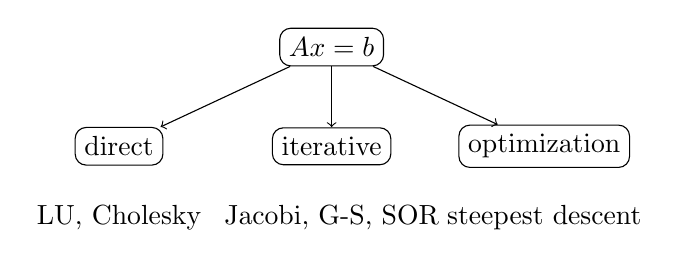
\begin{tikzpicture}[scale=0.9]
  \node[draw,rounded corners] (A) at (0,0) {$Ax=b$};
  \node[draw,rounded corners] (D) at (-3,-1.4) {direct};
  \node[draw,rounded corners] (I) at (0,-1.4) {iterative};
  \node[draw,rounded corners] (O) at (3,-1.4) {optimization};
  \draw[->] (A) -- (D); \draw[->] (A) -- (I); \draw[->] (A) -- (O);
  \node at (-3,-2.4) {LU, Cholesky};
  \node at (0,-2.4) {Jacobi, G-S, SOR};
  \node at (3,-2.4) {steepest descent};
\end{tikzpicture}
\caption{Linear systems can be solved by factorization, iteration, or minimization.}
\end{figure}

\section{Checklist}
\[
\begin{array}{c|c}
\text{Gauss} & \text{triangularize}\\
\text{pivoting} & \text{avoid small pivots}\\
\text{Cholesky} & \text{positive definite}\\
\text{chasing} & \text{tridiagonal}\\
\text{iteration} & \rho(B)<1\\
\text{SOR} & 0<\alpha<2\text{ for SPD}\\
\text{steepest descent} & \text{quadratic minimization}
\end{array}
\]
